This section contains some instructions and examples for using \LaTeX.

\subsection{You can add subsections}
You can use numbered subsections to structure your sections or $\backslash\texttt{paragraph}$ to separate paragraphs with a heading using only a few words, as used in Section~\ref{sec:introduction}.


\begin{enumerate}
	\item\label{item:1} This is an item in an enumeration.
    \begin{itemize}
    	\item This is an item of a unnumbered list. In this case, the lists are nested within each other.
    \end{itemize}
    \item\label{item:2} The second point in the enumerated list.
\end{enumerate}
%
I can refer to the element of the enumeration above as Point~\ref{item:1}.
If you refer to numbered items,~e.g. items from a list or figures or sections, always capitalize the name. 
For example, this is Section~\ref{sec:latex}.

\subsection{Figures}
You can include figures. You can include files, as done in Figure~\ref{fig:example}. 
Avoid including jpeg, gif or bmp files since these do not scale nicely. Again Figure~\ref{fig:example} is an example for that.

\begin{figure}[t]
   \centering
   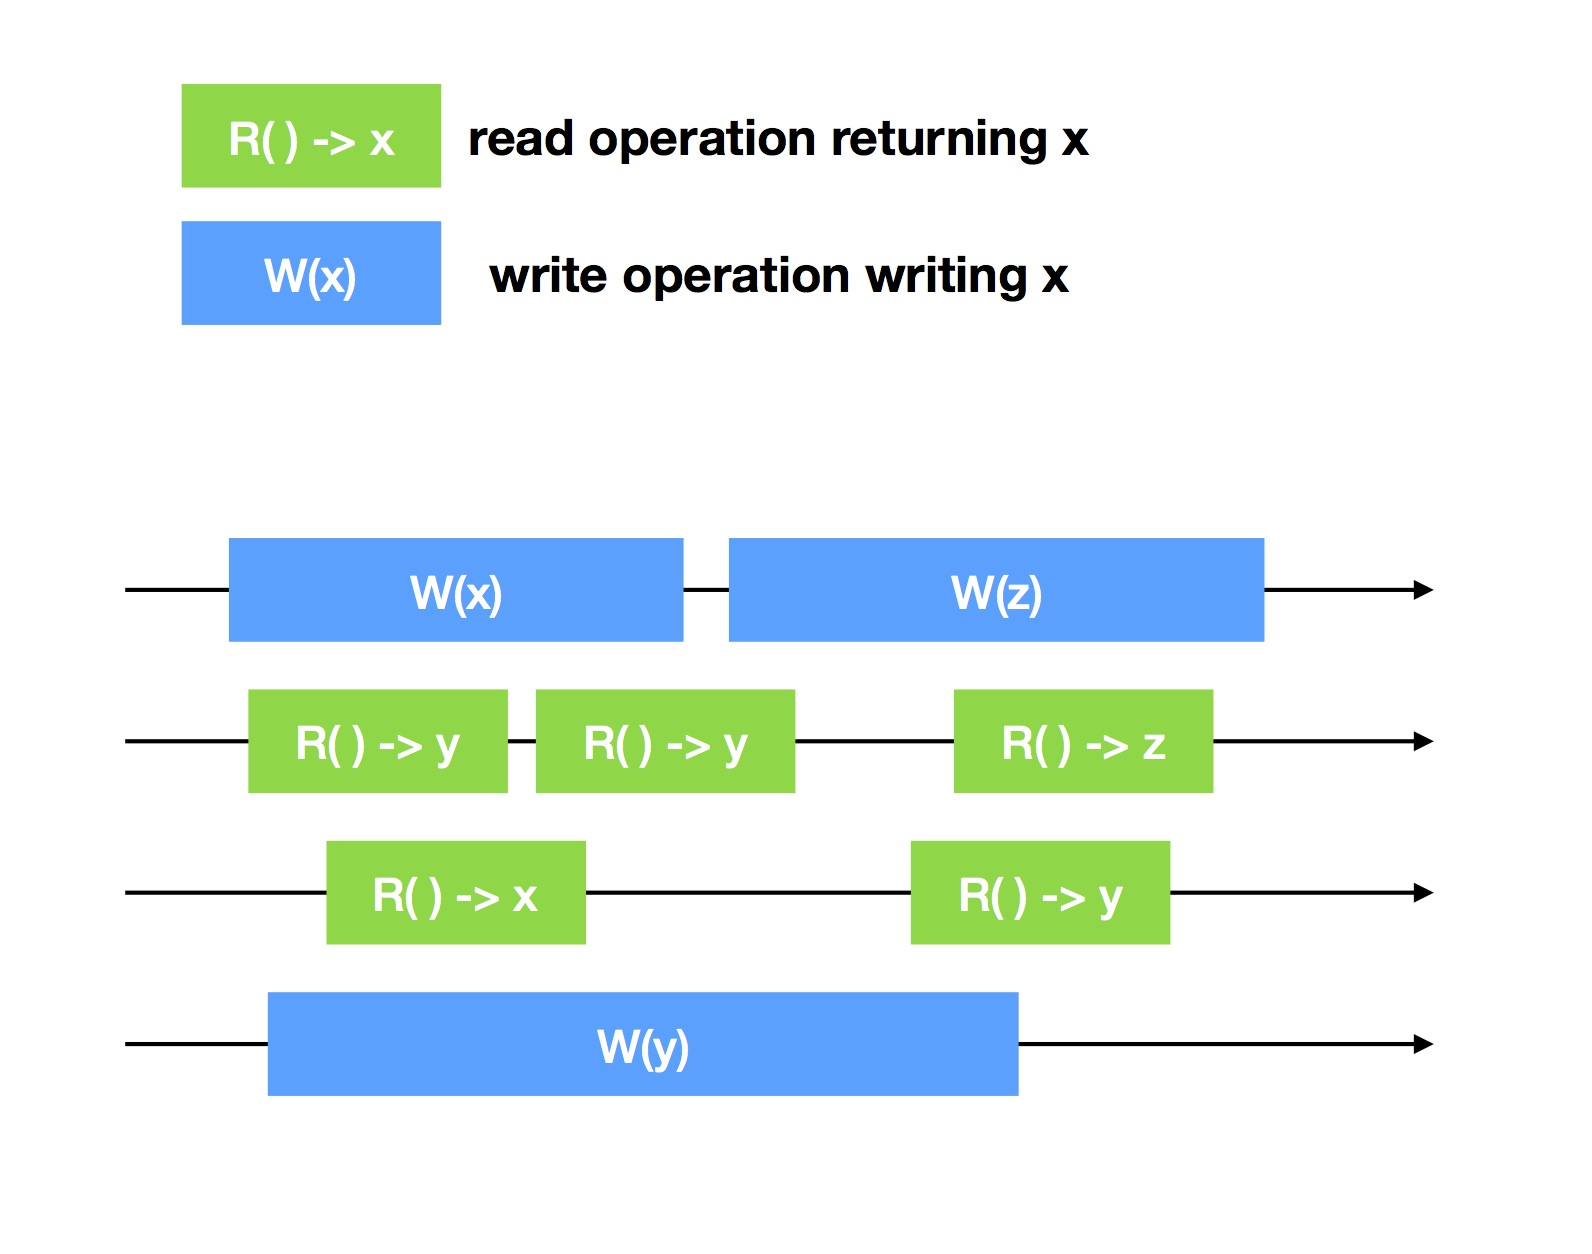
\includegraphics[width=\linewidth]{fig/RegisterOperations}
    \caption{Figure taken from~\cite{lecture}}
    \label{fig:example}
\end{figure}

You can create graphs from your experiment-data using \texttt{pgfplots}.
See the example in \texttt{tex/evaluation.tex} and documentation \url{http://pgfplots.sourceforge.net/pgfplots.pdf}.

\subsection{Other tips}
\begin{itemize}

\item Always use the tilde character between the number and unit, e.g. 100~Mbps or 53~ms. The tilde inserts a space, but prevents line break between the number and unit.

\item Never put SI units in italics. 

\item Do differentiate between bits (b) and bytes (B), and between powers of 10~(MB) and 2~(MiB).

\item Avoid things like: "We refer the reader to [42]." That is, don't use citations as nouns.
\end{itemize}

For further instructions on how to add \textbf{Tables, Algorithms, Theorems see acmguide.pdf}.
